\lab{Collective Communication}{Collective Communication in Parallel Programs}
\objective{Learn how to use collective communication to increase the efficiency of parallel programs}
\label{lab:MPI_Collective_Communication}

In the lab on the Trapezoidal Rule [Lab \ref{lab:MPI_Trapezoidal_Rule}], we worked to increase the efficiency of the trapezoidal rule by parallelizing the code and by load-balancing the parallel processes. However, the algorithm is still far from being optimized.

Look back at the summation that the root process (process 0) does. After each process independently calculates its estimate, the results must be compiled somehow, and the method we have chosen is rather inefficient. While the root process sums the data, the other processors sit idly. A more efficient algorithm would balance the work-load so that there are non-idling processes. Additionally, the root process is solely responsible for communicating with each of the other processes. The communication involved in parallel programs is usually a substantial bottleneck, and this is no exception. 
% TODO learn/explain why communication is such a huge bottleneck

Both of these problems can be somewhat corrected through what is called ``Collective Communication.'' Besides helping to alleviate load imbalances, however, collective communication has a more important purpose: it helps to optimize message passing among separate processes. Communication among processes is expensive. Because each message must be sent over some sort of network, we must minimize and optimize this inter-process communication.

There are two important principles to remember here:
\begin{enumerate}
\item[Load Balancing:]
A program is inefficient if it is not using all of the available resources (e.g., processes are idling because they are waiting for each other)
\item[Communication is Expensive:]
\emph{Broadcast} and \emph{Reduce} (two MPI functions we will introduce in this lab) are designed to optimize communication among the whole communicator. However, any sort of message passing is extremely expensive and one of the main obstacles to obtaining speedups when parallelizing an algorithm.
% TODO explain how efficiency actually **gets worse** if you add too many processors beause of the communication overhead
\end{enumerate}


\section*{Tree-Structured Computation}
Suppose we have eight processes, each with a number to be summed. Let the even ranked processes send their data to the odd process one greater than each respective process. The odd processes receive data from directly below them in rank. By so doing, we have in one time-step done half of the work.
% \begin{figure}[htbp]
% \centering
% \capstart

% Fast summation picture:
\begin{figure}
\centering
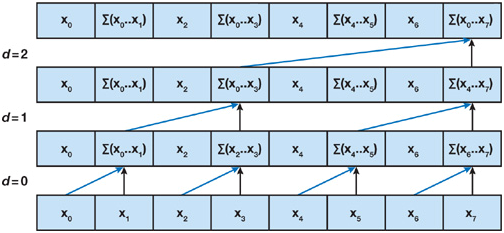
\includegraphics[width=.9\textwidth]{fastSum.png}
\caption{Tree structure in fast summation.}
\label{fig:fast_sum}
\end{figure}


From this point we can repeat the process with the odd processes, further partitioning them. A summation done in this manner creates a tree structure (see the figure [\ref{fig:fast_sum}]). MPI has implemented fast summations and much more in methods referred to as ``Collective Communication.'' The method shown in the figure is called \emph{Reduce}.

Furthermore, MPI has methods that can also distribute information in efficient ways. Imagine reversing the arrows in the figure [\ref{fig:fast_sum}]. This is MPI's \emph{Broadcast} function. We should note, though, that the image is a simplification of how MPI performs collective communication. In practice, it is different in every implementation, and is usually more efficient than the simplified example shown. MPI is designed to optimize these methods under the hood, and so we only need to worry about properly applying these functions.

Knowing this, let's take another look at the trapezoidal rule.


\section*{The Parallel Trapezoidal Rule 2.0}
Below is the code for our revised edition of the trapezoid rule. (This code requires that the number of trapezoids is evenly divisible by the the number of processes). The main change is that the statement \li{comm.Reduce(integral, total)} has replaced the entire if-else statement that was used to compile the results, including the for loop. Not only does the code look cleaner, it runs faster.

\lstinputlisting[style=FromFile]{trapParallel_2.py}

Some explanation is necessary for the call to \li{COMM.Reduce}. The first argument, \li{integral}, is the number which is going to be added up. This number is different for every process. The variable \li{total_buffer} will hold the result in the root process after this line runs. The parameter \li{op=MPI.SUM} tells the communicator to use the addition operator to combine the values.

The careful observer may have noticed from the figure \ref{fig:fast_sum} that in the end of the call to \li{Reduce}, only the root process holds the final summation. This brings up an important point: \emph{collective communication calls can return different values to each process}. This can be a ``gotcha'' if you are not paying attention.

So what can we do if we want the result of a summation to be available to all processes? Use the provided subroutine \li{AllReduce}. It does the same thing as \li{Reduce}, but it simultaneously uses each process as the root. That way, by the end of the summation, each process has calculated an identical sum. Duplicate work was done, but in the end, the result ends up on each process at the same time.

So when should we use \li{Reduce} and when should we use \li{AllReduce}? If it is unimportant for all processes to have the result, as is the case with the Trapezoidal Rule, using \li{Reduce} should be slightly faster than using \li{AllReduce}. On the other hand, if every process needs the information, \li{AllReduce} is the fastest way to go. We could come up with some other solutions to the situation, such as a call to \li{Reduce}, followed by a call to \li{Broadcast}, however these other solutions are always less efficient than just using one call to the collective communication routines. In the end, the less communications, the better.

% TODO (originally here from Jeremy's notes) Theoretically, Allreduce could be just as fast as Reduce. Insert Butterfly communication pattern here


\section*{Reduce(...) and Allreduce(...)}

\begin{description}
\item[Comm.Reduce(sendbuf, recvbuf, Op op=MPI.SUM, root=0)]
Reduces values on all processes to a single value on the root process.
Parameters:
\begin{description}
\item[sendbuf (array-like)] – address of send buffer
\item[recvbuf (array-like)] – address of recieve buffer (only significant in root process)
\item[op (MPI Op)] – reduce operation
\item[root (int)] – rank of root of operation
\end{description}
Example:
\lstinputlisting[style=FromFile]{Reduce_example.py}
\item[Comm.Allreduce(sendbuf, recvbuf, Op op=MPI.SUM)]
Reduces values on all processes to a single value on all processes.
Parameters:
\begin{description}
\item[sendbuf (array-like)] – address of send buffer
\item[recvbuf (array-like)] – address of recieve buffer (only significant in root process)
\item[op (MPI Op)] – reduce operation
\end{description}
Example:
Same as the example for Reduce except replace COMM.Reduce with COMM.Allreduce and remove the if statement. Notice that all process now have the “reduced” value.
\end{description}

The following table contains the predefined operations that can be used for the input parameters \emph{Op}. There are also methods that allow the creation of user-defined operations. Full documentation is found here: \url{http://mpi4py.scipy.org/docs/apiref/mpi4py.MPI.Op-class.html}.

TODO figure out how to format this table

% \begin{array}{\linewidth}{|L|L|}
% \hline
% \textbf{
% Name
% } & \textbf{
% Meaning
% }\\\hline

% MPI.MAX
%  & 
% maximum
% \\\hline

% MPI.MIN
%  & 
% minimum
% \\\hline

% MPI.SUM
%  & 
% sum
% \\\hline

% MPI.PROD
%  & 
% product
% \\\hline

% MPI.LAND
%  & 
% logical and
% \\\hline

% MPI.BAND
%  & 
% bit-wise and
% \\\hline

% MPI.LOR
%  & 
% logical or
% \\\hline

% MPI.BOR
%  & 
% bit-wise or
% \\\hline

% MPI.LXOR
%  & 
% logical xor
% \\\hline

% MPI.BXOR
%  & 
% bit-wise xor
% \\\hline

% MPI.MAXLOC
%  & 
% max value and location
% \\\hline

% MPI.MINLOC
%  & 
% min value and location
% \\\hline
% \end{array}


\begin{problem}
What is the difference between \li{Reduce} and \li{Allreduce}?
\end{problem}

\begin{problem}
Why is \li{Allreduce} faster than a \li{Reduce} followed by a \li{Bcast}?
\end{problem}



\section*{Parallelizing the Dot Product}
Calculating a dot product is a relatively simple task which does not need to be parallelized, but it makes a good example for introducing the other important collective communication subroutines. When provided two vectors, the dot product is the sum of the element wise multiplications of the two vectors:
\[
\textbf{u} \cdot \textbf{v} = \sum_{i=1}^{n} u_i v_i
\]

In order to parallelize this, we can divide up the work among different processors by sending pieces of the original vectors to different processors. Each processor then multiplies its elements and sums them. Finally, the local sums are summed using \li{Reduce}, which sums numbers distributed among many processes in \emph{O(log n)} time.

The code looks like this:

\lstinputlisting[style=FromFile]{dot.py}

The actual distributing of the data occurs with the calls to \li{Scatter}. \li{Scatter} takes an array, divides it up, and distributes one piece to each process. Afterward, the serial dot product (using \li{np.dot}) is run to calculate a local dot product within each process. Finally, \li{Reduce} is called to collect the results into the root process.

With this new algorithm and enough processors, the runtime approaches O(log n) time. To help understand how much faster this is compared to the original version, imagine that we have as many processors as we have items in each array: say, 1000. Then, each of these operations requires the same amount of time, the algorithm's runtime would run hypothetically something like this:

TODO figure out how to format this table

% \begin{array}{\linewidth}{|L|L|L|L|}
% \hline
% \textbf{
% Task vs Time
% } & \textbf{
% Serial Code
% } & \textbf{
% Point-to-Point mpi
% } & \textbf{
% Collective mpi
% }\\\hline

% Broadcast n = 1000
%  & 
% N/A
%  & 
% About 1000
%  & 
% About 10
% \\\hline

% Scatter x
%  & 
% N/A
%  & 
% About 1000
%  & 
% About 10
% \\\hline

% Scatter y
%  & 
% N/A
%  & 
% About 1000
%  & 
% About 10
% \\\hline

% Compute sum
%  & 
% 1000
%  & 
% 1
%  & 
% 1
% \\\hline

% Reduce result
%  & 
% N/A
%  & 
% About 1000
%  & 
% About 10
% \\\hline

% \textbf{Total}
%  & 
% \textbf{About 1000}
%  & 
% \textbf{About 4001}
%  & 
% \textbf{About 41}
% \\\hline
% \end{array}


The first column shows the serial dot product's time requirements. The final column shows the mpi-version. It is clear that the final version requires less time and that this number drops with the number of processors used. We simply cannot get this speed up unless we break out of the serial paradigm.

The middle column illustrates why we should use \emph{broadcast}, and \emph{scatter}, and \emph{reduce} over using \emph{n} \emph{send/recv} pairs in a for-loop. We do not include code for this variation. \emph{It turns out that using MPI in this fashion can actually run slower than the serial implementation of our dot product program.}



\section*{A Closer Look at Broadcast and Reduce}
Let's take a closer look at the call to \li{COMM.Bcast}. \li{Bcast} sends data from one process to all others. It uses the same tree-structured communication illustrated in the Fast Sum figure [\ref{fig:fast_sum}]. It takes for its first argument an array of data, which must exist on all processors. However, what is contained in that array may be insignificant. The second argument tells Bcast which process has the useful information. It then proceeds to overwrite any data in the arrays of all other processes.

Bcast behaves as if it is synchronous. ``Synchronous'' means that all processes are in sync with each other, as if being controlled by a global clock tick. For example, if all processes make a call to \li{Bcast} they will all be guaranteed to be calling the subroutine at basically the same time.

For all practical purposes, you can also think of \li{Reduce} as being synchronous. The difference is that Reduce only has one receiving process, and that process is the only process whose data is guaranteed to contain the correct value at completion of the call. To test your understanding of Reduce, suppose we are adding the number one up by calling \li{COMM.Reduce} on 100 processes, with the root being process 0. The documentation of \li{COMM.Reduce} tells us that the receive buffer of process 0 will contain the number 100. What will be in the receive buffer of process 1?

The answer is we don't know. The reduce could be implemented in one of several ways, dependent on several factors, and as a result it is non-deterministic. During collective communications such as \li{Reduce}, we have no guarantee of what value will be in the intermediate processes' receive buffer. More importantly, future calculations should never rely on this data except in process root (process \emph{0} in our case).


\begin{problem}
In our parallel implementation of the calculation of the dot product, \texttt{dotProductParallel\_1.py}, the number of processes must evenly divide the length of the vectors. Rewrite the code so that it runs regardless of vector length and number of processes (though for convenience, you may assume that the vector length is greater than the number of processes). Remember the principle of load balancing. Use Scatterv() to accomplish this.

% TODO add hint about how easy this is

\end{problem}

\begin{problem}
Alter your code from the previous exercise so that it calculates the supremum norm(the maximal element) of one of the vectors (choose any one). This will include changing the operator Op in the call to \li{Reduce}.
\end{problem}

\begin{problem}
Use \li{Scatter} to parallelize the multiplication of a matrix and a vector. There are two ways that this can be accomplished. Both use \li{Scatter} to distribute the matrix, but one uses \li{Bcast} to distribute the vector and \li{Gather} to finish while the other uses \li{Scatter} to segment the vector and finishes with \li{Reduce}. Outline how each would be done. Discuss which would be more efficient (hint: think about memory usage). Then, write the code for the better one. Generate an arbitrary matrix on the root node. You may assume that the number of processes is equal to the number of rows (columns) of a square matrix. Example code demonstrating scattering a matrix is shown below:

\lstinputlisting[style=FromFile]{matrix_scatter_example.py}
\end{problem}

